\section{Methodology}
% Plan (type T): 3.1 objective with two error terms (shift bias / estimation variance) + oracle weight;
% 3.2 adaptive side: whitened shift score (limitation i, Stale Source Statistics);
% 3.3 stable side: Stein weight + lemma + proposition (limitation ii, Noisy Batch Statistics);
% 3.4 assembled SourceStein for means and variances + cost.
In this section, we present \textbf{SourceStein}, an adaptive and stable rule that chooses the mixing weight of Equation~\ref{eq:mixing} separately for each test batch and each BN layer.
We first write the error of the mixed statistics as a sum of a shift bias and an estimation variance in Section~\ref{sec:shrinkage-problem}, which yields the best mixing weight in closed form.
After that, Section~\ref{sec:shift-score} estimates the unknown shift with a whitened shift score.
Then, Section~\ref{sec:stein-weight} turns the score into the Stein weight and states its risk guarantee.
Finally, Section~\ref{sec:sourcestein} applies the same rule to the variances and assembles the complete method.

\begin{figure*}[t]
    \centering
    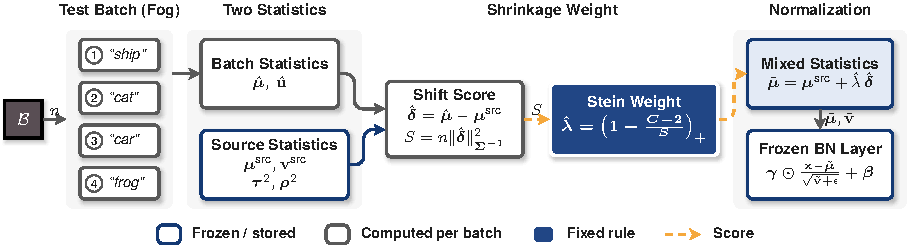
\includegraphics{figures/framework/main_figure.pdf}
    \caption{Overview of SourceStein at one BN layer. A test batch of $n$ fog-corrupted images yields the batch statistics $\hat{\boldsymbol{\mu}}, \hat{\mathbf{u}}$, while the frozen layer stores the source statistics $\boldsymbol{\mu}^{\text{src}}, \mathbf{v}^{\text{src}}$ and the between-sample variances $\boldsymbol{\tau}^2, \boldsymbol{\rho}^2$ measured once on training data. (1) The shift score $S$ measures the observed shift $\hat{\boldsymbol{\delta}}$ in units of the noise expected from $n$ samples. (2) The Stein weight $\hat{\lambda}$ keeps only the part of the shift that exceeds this noise. (3) The mixed statistics replace the stored ones inside the unchanged BN layer.}
    \label{fig:main-figure}
    \vspace{-6pt}
\end{figure*}

\subsection{Test-Time Statistics as a Shrinkage Problem} \label{sec:shrinkage-problem}
To choose $\lambda$ for a given batch, we first state what a good mixed mean should achieve.
Recall that $\boldsymbol{\mu}^{\text{tgt}}$ is the mean the layer would use with unlimited test data, and let $\boldsymbol{\delta} = \boldsymbol{\mu}^{\text{tgt}} - \boldsymbol{\mu}^{\text{src}}$ be the true shift and $\boldsymbol{\Sigma} = \operatorname{diag}(\boldsymbol{\tau}^2)$ the covariance of a single per-sample mean $\mathbf{m}_i$.
The batch mean $\hat{\boldsymbol{\mu}}$ then has covariance $\boldsymbol{\Sigma}/n$.
We measure the error of Equation~\ref{eq:mixing} in the noise units of the layer:
\begin{equation}\label{eq:risk}
\begin{aligned}
R(\lambda) &= \mathbb{E}\, n \big\|\boldsymbol{\mu}(\lambda) - \boldsymbol{\mu}^{\text{tgt}}\big\|^{2}_{\boldsymbol{\Sigma}^{-1}}\\
&= \underbrace{(1-\lambda)^{2}\,\Delta}_{\text{shift bias}} + \underbrace{\lambda^{2}\,C}_{\text{estimation variance}},
\end{aligned}
\end{equation}
where $\|\mathbf{x}\|^2_{\boldsymbol{\Sigma}^{-1}} = \mathbf{x}^{\top}\boldsymbol{\Sigma}^{-1}\mathbf{x}$ and $\Delta = n\|\boldsymbol{\delta}\|^2_{\boldsymbol{\Sigma}^{-1}}$ is the whitened shift.
Specifically, the first term is the shift bias of keeping the source statistics, and the second is the estimation variance of trusting $n$ samples.
Setting the derivative to zero yields the best weight of the family:
\begin{equation}\label{eq:oracle}
\lambda^{\star} = \frac{\Delta}{\Delta + C}, \qquad R(\lambda^{\star}) = \frac{C\,\Delta}{\Delta + C}.
\end{equation}
This oracle weight moves toward the batch as the shift or the batch increases, and remains near the source when the shift is small compared with the noise.
In contrast, the weight $n/(n+N)$ of Prior-BN equals $\lambda^{\star}$ only when $\|\boldsymbol{\delta}\|^2_{\boldsymbol{\Sigma}^{-1}} = C/N$, \ie for one shift size per pseudo sample size.
TBN incurs $R(1) = C$ at each shift, and the source model incurs $R(0) = \Delta$, which is unbounded in the shift.

\subsection{Adaptive Mixing via a Whitened Shift Score} \label{sec:shift-score}
To counter stale source statistics, the weight must respond to the shift $\Delta$, which is unknown at test time.
We estimate it from the test batch statistics through the observed shift $\hat{\boldsymbol{\delta}} = \hat{\boldsymbol{\mu}} - \boldsymbol{\mu}^{\text{src}}$ through the shift score:
\begin{equation}\label{eq:shift-score}
S = n\,\big\|\hat{\boldsymbol{\delta}}\big\|^{2}_{\boldsymbol{\Sigma}^{-1}} = n \sum_{c=1}^{C} \frac{(\hat{\mu}_c - \mu^{\text{src}}_c)^{2}}{\tau^{2}_c},
\end{equation}
whose expectation is $\mathbb{E}[S] = \Delta + C$: the true shift plus the noise of $n$ samples.
Specifically, the score requires the noise level $\boldsymbol{\tau}^2$, which a batch of one image cannot estimate.
Therefore, we measure it once on the training data, as the variance of the per-sample means $\mathbf{m}_i$ over $5{,}000$ training images, and store it together with $\boldsymbol{\mu}^{\text{src}}$.
Under this choice, a shift that is large compared with the training spread of single images drives $S$ far above $C$, and the weight can follow it.
In contrast, a clean batch has $\mathbb{E}[S] = C$ up to the train--test gap of the source statistics, and its score remains close to the number of channels.

\textbf{Choice of the noise level.} The source noise level is an assumption: a corruption can change the spread of single images as well as their mean.
We keep it because it is available for each batch size, including $n{=}1$, while a noise level estimated from $n$ test samples is itself a noisy ratio for small $n$.
Section~\ref{sec:ablation-study} compares both choices, and Appendix~\ref{apdx:synthetic} shows what a misestimated noise level costs in simulation.

\subsection{Stable Mixing with the Stein Weight} \label{sec:stein-weight}
With the shift measured by $S$, the plug-in of Equation~\ref{eq:oracle} would be $1 - C/S$.
However, $S$ is noisy when $n$ is small, and a plug-in weight inherits this noise exactly where the estimation variance matters most.
Therefore, we rely on the following classical result, in which the shrinkage target is the source mean:
\begin{lemma}[James--Stein Estimator \cite{James-Stein}]\label{lemma:james-stein}
Let $\mathbf{z} \sim \mathcal{N}(\boldsymbol{\theta}, \mathbf{I}_C)$ with $C \ge 3$, let $\mathbf{a} \in \mathbb{R}^{C}$ be fixed, and let $s = \|\mathbf{z} - \mathbf{a}\|^2$. Then $\hat{\boldsymbol{\theta}} = \mathbf{a} + (1 - (C-2)/s)(\mathbf{z} - \mathbf{a})$ has risk $\mathbb{E}\|\hat{\boldsymbol{\theta}} - \boldsymbol{\theta}\|^2 = C - (C-2)^2\,\mathbb{E}[1/s]$, and clipping the factor at zero does not increase the risk \cite{Efron-Morris}.
\end{lemma}
Applying the lemma to the whitened batch mean $\mathbf{z} = \sqrt{n}\,\boldsymbol{\Sigma}^{-1/2}\hat{\boldsymbol{\mu}}$ with $\mathbf{a} = \sqrt{n}\,\boldsymbol{\Sigma}^{-1/2}\boldsymbol{\mu}^{\text{src}}$, for which $s = S$, yields the Stein weight:
\begin{equation}\label{eq:stein-weight}
\hat{\lambda} = \Big(1 - \frac{C-2}{S}\Big)_{+},
\end{equation}
where $(x)_+ = \max(x, 0)$.
As a result, the weight is zero until the shift score exceeds $C-2$ and approaches one as the shift dominates the noise.

\textbf{One weight per layer.} The $C$ channels of a layer share one weight, because the lemma pools their evidence: a shift that is small in each channel but present in many of them still increases $S$.
In contrast, a separate weight per channel would base each decision on a single noisy value, and the guarantee below requires $C \ge 3$.
However, the price is that channels with different shifts receive the same weight, which Section~\ref{sec:ablation-study} examines.
The risk of the Stein weight compares with the two fixed extremes and with the oracle as follows:
\begin{proposition}\label{prop:risk}
Assume $\hat{\boldsymbol{\mu}} \sim \mathcal{N}(\boldsymbol{\mu}^{\text{tgt}}, \boldsymbol{\Sigma}/n)$ with $C \ge 3$. Then the Stein weight satisfies $R(\hat{\lambda}) \le C - (C-2)^2/(C + \Delta)$, which is \textbf{below the risk $C$ of TBN} for each shift, and $R(\hat{\lambda}) - R(\lambda^{\star}) \le 4(C-1)/(C+\Delta) < 4$.
\end{proposition}
Specifically, the first bound follows from Lemma~\ref{lemma:james-stein} and Jensen's inequality $\mathbb{E}[1/S] \ge 1/\mathbb{E}[S]$, and the second subtracts Equation~\ref{eq:oracle} (see Appendix~\ref{apdx:proof} for the proof).
Measured per channel, the excess over the oracle is below $4/C$, which is small for layers with 16 to 128 channels.

\textbf{Relation to Prior-BN.} Each Stein weight corresponds to a pseudo sample size $\hat{N} = n(1-\hat{\lambda})/\hat{\lambda}$ of Prior-BN, chosen per layer and per batch.
Specifically, a batch whose shift score is close to $C$ receives a very large $\hat{N}$ and keeps the source statistics, while a batch with a large score receives a small $\hat{N}$ and moves toward its own statistics.
Prior-BN, in contrast, uses one $N$ for all layers, batches and corruptions.

\textbf{Discussion.} The Stein weight has an empirical Bayes reading \cite{Efron-Morris}: $(C-2)/S$ estimates the share of the observed shift that is noise, and $\hat{\lambda}$ keeps the rest.
Moreover, the choice of the shrinkage target matters here.
Prior uses of Stein shrinkage in normalization layers shrink toward a centre computed from the same batch during training \cite{JS-Norm, Stein-BN-Adv}, which reduces noise but cannot correct a shift.
SourceStein instead shrinks toward the source statistics, so that the target contains the knowledge of the training data and the batch only has to supply the evidence of a shift.

\begin{algorithm}[t]
  \captionsetup{labelformat=default,labelsep=colon,name=Algorithm}
  \caption{Normalization with SourceStein}
  \label{alg:sourcestein}
\begin{algorithmic}
  \STATE {\bfseries Input:} test features $\{\mathbf{h}_i\}_{i=1}^{n}$ at one BN layer; stored $\boldsymbol{\mu}^{\text{src}}, \mathbf{v}^{\text{src}}, \boldsymbol{\tau}^2, \boldsymbol{\rho}^2, \boldsymbol{\gamma}, \boldsymbol{\beta}$.
  \STATE \CommentBelow{batch statistics (Equation~\ref{eq:batch-stats})}
  \STATE $\mathbf{m}_i \leftarrow \operatorname{mean}_{hw}\mathbf{h}_i$, \ $\mathbf{u}_i \leftarrow \operatorname{mean}_{hw}(\mathbf{h}_i - \boldsymbol{\mu}^{\text{src}})^2$
  \STATE $\hat{\boldsymbol{\mu}} \leftarrow \operatorname{mean}_i \mathbf{m}_i$, \ $\hat{\mathbf{u}} \leftarrow \operatorname{mean}_i \mathbf{u}_i$
  \STATE \tikzmk{algA}\CommentBelow{shift scores and Stein weights}
  \STATE $S_\mu \leftarrow n\sum_c (\hat{\mu}_c - \mu^{\text{src}}_c)^2/\tau^2_c$
  \STATE $S_u \leftarrow n\sum_c (\hat{u}_c - v^{\text{src}}_c)^2/\rho^2_c$
  \STATE $\hat{\lambda}_\mu \leftarrow (1 - \frac{C-2}{S_\mu})_+$, \ $\hat{\lambda}_u \leftarrow (1 - \frac{C-2}{S_u})_+$\tikzmk{algB}
  \STATE \CommentBelow{mixed statistics (Equation~\ref{eq:sourcestein})}
  \STATE $\tilde{\boldsymbol{\mu}} \leftarrow \boldsymbol{\mu}^{\text{src}} + \hat{\lambda}_\mu(\hat{\boldsymbol{\mu}} - \boldsymbol{\mu}^{\text{src}})$
  \STATE $\tilde{\mathbf{u}} \leftarrow \mathbf{v}^{\text{src}} + \hat{\lambda}_u(\hat{\mathbf{u}} - \mathbf{v}^{\text{src}})$
  \STATE $\tilde{\mathbf{v}} \leftarrow \max(\tilde{\mathbf{u}} - (\tilde{\boldsymbol{\mu}} - \boldsymbol{\mu}^{\text{src}})^2, 10^{-5})$
  \STATE {\bfseries return} $\boldsymbol{\gamma} \odot (\mathbf{h}_i - \tilde{\boldsymbol{\mu}})/\sqrt{\tilde{\mathbf{v}} + \epsilon} + \boldsymbol{\beta}$ for each $i$.
\end{algorithmic}
\boxit[Stein]{PhaseABg}{algA}{algB}
\end{algorithm}

\subsection{SourceStein} \label{sec:sourcestein}
Combining the shift score with the Stein weight, SourceStein treats the variance in the same way as the mean.
The per-sample second moments $\mathbf{u}_i$ have mean $\mathbf{v}^{\text{src}}$ on source data and between-sample variances $\boldsymbol{\rho}^2$, which we store with $\boldsymbol{\tau}^2$.
For each BN layer and each test batch, SourceStein computes:
\begin{equation}\label{eq:sourcestein}
\begin{aligned}
\tilde{\boldsymbol{\mu}} &= \boldsymbol{\mu}^{\text{src}} + \hat{\lambda}_{\mu}\,(\hat{\boldsymbol{\mu}} - \boldsymbol{\mu}^{\text{src}}),\\
\tilde{\mathbf{u}} &= \mathbf{v}^{\text{src}} + \hat{\lambda}_{u}\,(\hat{\mathbf{u}} - \mathbf{v}^{\text{src}}),\\
\tilde{\mathbf{v}} &= \max\!\big(\tilde{\mathbf{u}} - (\tilde{\boldsymbol{\mu}} - \boldsymbol{\mu}^{\text{src}})^{2},\ 10^{-5}\big),
\end{aligned}
\end{equation}
where $\hat{\lambda}_{\mu}$ is Equation~\ref{eq:stein-weight} with $(\hat{\boldsymbol{\mu}}, \boldsymbol{\mu}^{\text{src}}, \boldsymbol{\tau}^2)$ and $\hat{\lambda}_{u}$ is the same rule with $(\hat{\mathbf{u}}, \mathbf{v}^{\text{src}}, \boldsymbol{\rho}^2)$.
The layer then normalizes with $\tilde{\boldsymbol{\mu}}$ and $\tilde{\mathbf{v}}$ in Equation~\ref{eq:bn}, and the next layer sees the adapted features.
When both weights are one, Equation~\ref{eq:sourcestein} is equivalent to the batch statistics of Equation~\ref{eq:batch-stats}; when both are zero, it is equivalent to the source model.
Algorithm~\ref{alg:sourcestein} lists all steps of SourceStein for one layer.

\textbf{Cost.} SourceStein requires one pass over $5{,}000$ unlabelled training images to store $\boldsymbol{\tau}^2$ and $\boldsymbol{\rho}^2$, and no labels, gradients or hyperparameters.
At test time it adds $O(nCHW)$ operations per layer, the same order as computing the batch statistics; further implementation details are in Appendix~\ref{apdx:impl-details}.
